%%
% BIThesis 研究生学位论文模板 The BIThesis Template for Graduate Thesis
% This file has no copyright assigned and is placed in the Public Domain.
% Compile with: xelatex -> biber -> xelatex -> xelatex
%%

% 请勿删除下面两行注释,以免影响编译。
% !TeX program = xelatex
% !BIB program = biber

% 硕士论文模板 type=master
% 博士论文模板 type=doctor
% 开启盲审格式 blindPeerReview=true (如:[type=master,blindPeerReview=true])
% 开启双面打印模式 twoside=true (如:[type=master,twoside=true])
%     在双面打印模式下,需要放在奇数页的页面后会自动插入一个空白页,以方便直接在打印机上“双面打印”。
%
% 在 Linux 和 macOS 系统下,LaTeX 发行版默认使用的中文字体和 Windows 系统下的字体不同。
% 如果想要获得与 Word 文档相同的效果,请参阅在线帮助 https://bithesis.bitnp.net/faq/word-font.html
%
% **更多使用说明请参考 bithesis.pdf **

\documentclass[type=master,twoside=false]{bithesis}

% 此处仅列出常用的配置。全部配置用法请见「bithesis.pdf」手册。
\BITSetup{
  cover = {
    %% 使用以下参数来自定义封面日期
    date = ,
    autoWidthPadding = 0.25em,
  },
  info = {
    % 想要删除某项封面信息,直接删除该项即可。
    % 想要让某项封面信息留空(但是保留下划线),请传入空白符组成的字符串,如"{~}"。
    % 如需要换行,则用 “\\” 符号分割。
    classification = ,
    UDC = ,
    title = LLMalMorph:论使用大型语言模型生成恶意软件变体的可行性,
    % 如需覆盖竖排标题,请配置以下选项。
    % 下面的例子展示了如何在竖排标题中使用垂直或者旋转的英文。
    % verticalTitle = {形状记忆聚氨酯{L } {T } {X }的合成 \rotatebox[origin=c]{-90}{Feng Kaiyu} 及其在织物中的应用},
    titleEn = {LLMalMorph: On The Feasibility of Generating Variant Malware using Large-Language-Models},
    author = ,
    authorEn = ,
    studentId = ,
    school = ,
    schoolEn = ,
    supervisor = ,  % 指导教师
    supervisorEn = ,
    chairman = ,  % 答辩委员会主席
    chairmanEn = ,
    % -------------
    % 请按自身研究生类型填写以下项目
    %
    % --- 学术型 ---
    % degreeType = academic,
    % degree = 工学博士,  % 申请学位
    % degreeEn = Doctor of Engineering,
    % major = 材料科学与工程,  % 一级学科
    % majorEn = Materials Science and Engineering,
    %
    % --- 专业型 ---
    degreeType = professional,
    industrialMentor = ,  % 行业合作导师
    industrialMentorEn = ,
    degree = ,  % 申请类别
    degreeEn = {},
    major = ,  % 学位领域
    majorEn = ,
    % -------------
    %
    % 如果想要手动控制盲审模式下的隐藏信息,可以使用宏 \SecretInfo{}。使用方式有两种,如:
    % major = \SecretInfo{材料科学与工程} 可以得到 ******* (用等量的替换符号替代)
    % major = \SecretInfo{材料科学与工程}[ABCDEF] 可以得到 ABCDEF (用你自定义的内容替代)
    %
    defenseDate = ,
    defenseDateEn = {},
    keywords = {},
    keywordsEn = ,
    %
    % 必要时置于封面右上角,并按照国家规定进行标记。
    % classifiedLevel = 密级\BigStar 保密期限,
    %
    % 特别类型——工程硕博士专项
    % 工程硕博士专项 = true,
    % 特别类型——交叉研究方向(一般不用勾选)
    % crossResearch = true,
    % 特别类型——政府项目留学生(一般不用勾选)
    % internationalStudentUGP = true,
    % 以上三个选项不勾选时将会隐藏显示。
  },
  % 在目录页中不显示摘要和主要符号对照表的标题。
  TOC = {
    abstract = false,
    abstractEn = false,
    symbols = false,
  },
  style = {
    pageVerticalAlign = top,
    % 开启 Windows 平台下的中易宋体伪粗体。
    % windowsSimSunFakeBold = true,
    % 开启该选项后,将用 Times New Roman 的开源字体 TeX Gyre Termes 作为正文字体。
    % 这个选项适用于以下情况:
    % 1. 不想在系统中安装 Times New Roman。
    % 2. 在 Linux/macOS 下遇到 `\textsc` 无法正常显示的问题。
    % betterTimesNewRoman = true,
  },
  publications = {
    % 以下两个选项将影响「攻读学位期间发表论文与研究成果清单」中名称列表的省略阈值。
    % 一般来说,如果你在全部文献中最低排在第四位,建议你将两个值都设置为大于等于 4 的值。
    % 更详细的说明请见手册。
    maxbibnames = 10,
    minbibnames = 10,
    % 「攻读学位期间发表论文与研究成果清单」默认按学校要求,“按发表的时间顺序列出”。
    % 如需调整,可修改以下选项,详见 https://bithesis.bitnp.net/faq/bib-sort.html
    % sorting = false
  },
  % 采用章节标题级别的附录格式
  appendices / chapterLevel = true,
  const = {
    % 关于题名页的字段名称,截至2025年三月末,以下几项规定不完全一致:
    %     Word 模板(学位论文模版-{学术型,专业型}-2025.doc)、研函〔2018〕60号《北京理工大学研究生学位论文撰写规范》、GB/T 7713.1—2006《学位论文编写规则》
    % 目前的默认值按照 Word 模板,可能需要手动调整。
    % 例如取消注释下一行,会将「申请学位/类别」改为「申请学位级别」。
    % info / degree = {申\hspace{0.45ex}请\hspace{0.45ex}学\hspace{0.45ex}位\hspace{0.45ex}级\hspace{0.45ex}别},
    % 详见 https://bithesis.bitnp.net/faq/edit-const.html
  },
  misc = {
    % 关闭后,链接会用多种颜色表示,便于检查。
    % 无论是否开启,都不会影响打印效果。
    hideLinks = true,
    % 微调表格行间距
    tabularRowSeparation = 1.6,
  }
}

% 大部分关于参考文献样式的修改,都可以通过此处的选项进行配置。
% 详情请搜索「biblatex-gb7714-2015 文档」进行阅读。
\usepackage[
  defernumbers=true,
  backend=biber,
  style=gb7714-2015,
  gbalign=gb7714-2015,
  gbnamefmt=lowercase,
  gbpub=false,
  gbannote=true,
  gbpunctin=false,
  doi=false,
  url=false,
  eprint=false,
  isbn=false,
]{biblatex}

% 添加参考文献
\addbibresource{reference/main.bib}
% 攻读学位期间发表论文与研究成果清单,详细使用方法见 `chapters/pub.tex`。
%\addbibresource{reference/pub.bib}


\usepackage{graphicx}
\usepackage{tabularx}
\usepackage{ragged2e}
\usepackage[linesnumbered,ruled,vlined]{algorithm2e}

\begin{document}

% 封面绘制
\MakeCover

% 打印书脊
%\MakePaperBack

% 中文信息与英文信息
%\MakeTitle

% 论文原创性声明和使用授权
%\MakeOriginality

%%%%%%%%%%%%%%%%%%%%%%%%%%%%%%
%% 前置部分
%%%%%%%%%%%%%%%%%%%%%%%%%%%%%%
\frontmatter

% 摘要
%%
% BIThesis 研究生学位论文模板 The BIThesis Template for Graduate Thesis
% This file has no copyright assigned and is placed in the Public Domain.
%%

\begin{abstract}
Large Language Models (LLMs) have transformed software development and automated code generation. Motivated by these advancements, this paper explores the feasibility of LLMs in modifying malware source code to generate variants. We introduce LLMalMorph, a semi-automated framework that leverages semantical and syntactical code comprehension by LLMs to generate new malware variants. LLMalMorph extracts function level information from the malware source code and employs custom-engineered prompts coupled with strategically defined code transformations to guide the LLM in generating variants without resource-intensive fine-tuning. To evaluate LLMalMorph, we collected 10 diverse Windows malware samples of varying types, complexity and functionality and generated 618 variants. Our thorough experiments demonstrate that it is possible to reduce the detection rates of antivirus engines of these malware variants to some extent while preserving malware functionalities. In addition, despite not optimizing against any Machine Learning(ML)-based malware detectors, several variants also achieved notable attack success rates against an ML-based malware classifier. We also discuss the limitations of current LLM capabilities in generating malware variants from source code and assess where this emerging technology stands in the broader context of malware variant generation.
\end{abstract}

\begin{abstractEn}
大型语言模型(LLMs)已经改变了软件开发和自动化代码生成。受这些进展的激励,本文探索了LLMs修改恶意软件源代码以生成变种的可行性。我们引入了LLMalMorph,这是一个半自动化框架,它利用LLMs对代码的语义和语法理解来生成新的恶意软件变种。LLMalMorph从恶意软件源代码中提取函数级信息,并采用定制设计的提示词结合策略性定义的代码转换,来指导LLM生成变种,而无需资源密集型的微调。为了评估LLMalMorph,我们收集了10个不同类型、复杂度和功能的多样化Windows恶意软件样本,并生成了618个变种。我们详尽的实验表明,在保持恶意软件功能的同时,可以在一定程度上降低这些恶意软件变种对防病毒引擎的检测率。此外,尽管没有针对任何基于机器学习(ML)的恶意软件检测器进行优化,一些变种在对抗一个基于ML的恶意软件分类器时也取得了显著的攻击成功率。我们还讨论了当前LLM在从源代码生成恶意软件变种方面的能力局限性,并评估了这项新兴技术在更广泛的恶意软件变种生成背景下的现状。
\end{abstractEn}


% 制作目录
\MakeTOC

% 插图目录
\listoffigures
% 表格目录
\listoftables

% 主要符号对照表
%%
% BIThesis 研究生学位论文模板 The BIThesis Template for Graduate Thesis
% This file has no copyright assigned and is placed in the Public Domain.
%%

\begin{symbols}
  \item[BIT] 北京理工大学的英文缩写
  \item[\LaTeX] 一个很棒的排版系统
  \item[\LaTeXe] 一个很棒的排版系统的最新稳定版
  \item[ctex] 成套的中文\LaTeX{}解决方案,由一帮天才们开发
  \item[$ e^{\pi{}i}+1=0$] 一个集自然界五大常数一体的炫酷方程
\end{symbols}


\mainmatter

% 请根据论文内容,按照顺序添加章节。
%%
% BIThesis 研究生学位论文模板 The BIThesis Template for Graduate Thesis
% This file has 否 copyright assigned and is placed in the Public Domain.
%%

\chapter{引言}
恶意软件(Malware)继续随着技术的快速扩张而激增。到2025年,网络犯罪造成的损失预计将达到每年10.5万亿美元~\parencite{PIA2024}。每秒大约发生19万起新的恶意软件事件~\parencite{AVG2024},而2024年勒索软件的平均赎金要求预计将达到每次攻击273万美元,较往年急剧上升~\parencite{Sophos2024}。尽管经过数十年的研究和缓解努力,这些数字突显了恶意软件研究在当今不断演变的威胁环境中的紧迫重要性。

现代最具变革性的AI技术之一是大型语言模型(LLMs),它在自然语言处理(NLP)~\parencite{Dubey2024,Kedia2021,Jiang2023}、代码生成~\parencite{Hou2023,MAI2024,Roziere2023,Zhu2024,Lozhkov2024,Huang2024}以及代码编辑和重构等软件工程任务~\parencite{Cassano2024,Guo2024,Cordeiro2024}中展现了非凡的能力。鉴于这些优势和进步,利用LLMs进行恶意软件源代码转换是自然的发展。最近一项针对全球行业1800名安全负责人的调查\parencite{Darktrace2024}发现,74\%的人正经历着显著的AI驱动的威胁,60\%的人感觉准备不足,无法抵御这些威胁。尽管当前的模型仅从文本生成功能完整的恶意软件存在显著局限性,但研究表明它们可以生成恶意行为者能够组装成可操作恶意软件的代码片段\parencite{Botacin2023}。LLM能力的进步与恶意软件威胁的演变相结合,为对手使用这些模型创建新恶意软件并将现有代码库变异成更难以捉摸和更具破坏性的变种铺平了道路。尽管恶意软件源代码比二进制文件更难获取,但能够访问源代码的对手,例如恶意软件作者、泄露存储库的用户或修改开源恶意软件的人,仍然可以利用LLMs生成新的、更难检测的变种。这些模型使攻击者能够持续精进和扩展其武器库,从而大规模增加恶意活动的持久性和规避性。

\section{先前的研究}
先前的研究提出了各种创建恶意软件变种的方法\parencite{Botacin2023,Qiao2022,Choi2019,Lucas2021,Ming2017,Ling2024,Digregorio2024}。然而,这些方法在至少以下一个方面表现出局限性(如表\ref{tab:1.1}所示)(A) 大多数现有方法没有利用LLMs来转换恶意软件的源代码\parencite{Qiao2022,Choi2019,Lucas2021,Ming2017,Ling2024,Digregorio2024};(B) 大多数方法依赖迭代算法来生成恶意软件变种\parencite{Qiao2022,Choi2019,Lucas2021}, \parencite{Ling2024}, \parencite{Digregorio2024};(C) 使用LLMs进行变种生成的方法,直接从成功率低的提示词开始\parencite{Botacin2023}。此外,尚不清楚生成的恶意软件在规避广泛使用的防病毒引擎方面是否表现更优。鉴于目前的情况,我们的工作引入了一种与现有恶意软件变种生成方法截然不同的方法。与大多数先前主要依赖基于对抗性机器学习或基于搜索的方法的研究不同,我们的方法独特地利用LLMs在源代码级别进行操作。基本上,它从恶意软件源代码开始,以高成功率和最少的手动工作生成变种。此外,我们的方法不需要迭代训练或基于搜索的优化,这使其与现有的恶意软件转换方法根本不同。因此,我们提出了一个尚未充分探索的新研究方向。

\begin{table}[htbp]
	\centering
	\caption{与先前研究的对比}
	\label{tab:1.1}
	\begin{tabular*}{\textwidth}{@{\extracolsep{\fill}}ccccc}
		\toprule
		方法 & 源代码 & LLM使用 & 无需训练或迭代 & 逃逸提升 \\
		\midrule
		{\parencite{Qiao2022}} & 否 & 否 & 否 & 是 \\
		{\parencite{Digregorio2024}} & 否 & 否 & 否 & 是 \\
		{\parencite{Lucas2021}} & 否 & 否 & 否 & 是 \\
		{\parencite{Ling2024}} & 否 & 否 & 否 & 是 \\
		{\parencite{Ming2017}} & 否 & 否 & 是 & 是 \\
		{\parencite{Choi2019}} & 是 & 否 & 否 & 是 \\
        {\parencite{Botacin2023}} & 否 & 是 & 是 & 否 \\
        LLMalMorph & 是 & 是 & 是 & 是 \\
		\bottomrule
	\end{tabular*}
\end{table}

\section{问题描述}
鉴于现有方法的局限性以及LLMs(特别是代码生成方面)的最新进展,我们旨在回答以下问题——我们能否利用预训练LLMs的生成能力,无需额外微调,来开发一个半自动化且高效的框架,以生成保留功能语义的恶意软件变种,这些变种能够规避广泛使用的防病毒引擎和机器学习分类器?

\section{我们的方法}
在本文中,我们对上述问题给出了肯定的回答。我们设计、实现并评估了LLMalMorph——一个专门用于生成用C/C++编写的Windows恶意软件功能变种的框架。我们只专注于Windows恶意软件,因为它在消费者和企业环境中广泛使用,仍然是恶意软件最常针对的操作系统\parencite{AVG2024OS}, \parencite{Statcounter2024}。

LLMalMorph结合了自动化代码转换和人工监督来生成恶意软件变种。该框架利用一个开源的LLM,应用精心设计的转换策略和提示词工程,在保持结构和功能完整性的同时,高效地修改恶意软件组件。人机协同(human-in-the-loop)过程处理复杂转换和多文件恶意软件中的错误,允许进行调试和配置调整。这种半自动化方法也使我们能够量化基于LLM从源代码生成恶意软件变种中的人力投入。

\section{实验和分析}
我们选择了10个不同复杂度的恶意软件样本,使用6种代码转换策略结合一个LLM生成了618个变种。我们使用主要依赖基于签名的检测和静态分析的引擎的VirusTotal\footnote{https://www.VirusTotal.com/gui/home}和Hybrid Analysis\footnote{https://hybrid-analysis.com/}评估了防病毒(AV)检测率,并测试了语义保留性。代码优化(Code Optimization)策略在两种工具上均持续实现了较低的检测率。平均而言,相对于每个样本的基准检测率,LLMalMorph在VirusTotal上将简单样本的检测率降低了31\%,将三个更复杂样本的检测率降低了10\%至15\%;在Hybrid Analysis上,与各自基准相比,四个样本的检测率降低了8\%至13\%。除了AV工具外,我们还在一个基于机器学习(ML)的恶意软件分类器上评估了LLMalMorph,并观察到在特定样本上,优化(Optimization)策略和安全(Security)策略取得了较高的攻击成功率(分别高达89\%和91\%)。诸如优化、安全和Windows API修改等策略需要更多手动编辑,其中Windows和安全策略需要更高的调试投入。值得注意的是,四个样本中超过66\%的规避型变种保留了其语义,这证明了LLMalMorph生成功能规避型恶意软件的能力。

\section{贡献}
总结而言,我们有以下贡献:

• 我们设计并实现了LLMalMorph,一个实用的Windows恶意软件变种生成框架,它使用一个开源的LLM和基于提示词(prompt-based)的代码转换。

• 我们在LLMalMorph中设计了一个人机协同(human-in-the-loop)机制,以解决LLM在调试多文件恶意软件源代码和项目级配置方面的局限性。

• 我们进行了广泛的实验,从10个样本生成了618个恶意软件变种,并评估了它们在VirusTotal和Hybrid Analysis上的检测率和语义保留性,以及在一个机器学习分类器(ML Classifier)上的攻击成功率。

• 我们使用代码编辑工作量(code editing workload)比较了不同代码转换策略的有效性,并讨论了LLM所犯错误的类型。

\section{开源}
LLMalMorph框架及其所有相关组件可在Github\footnote{https://github.com/AJAkil/LLMalMorph}找到。
%%
% BIThesis 研究生学位论文模板 The BIThesis Template for Graduate Thesis
% This file has no copyright assigned and is placed in the Public Domain.
%%

\chapter{具体研究内容}

具体研究内容是学位论文的主要部分,是研究结果及其依据的具体表述,是研究能力的集中体现,一般应包括第2章、第3章至结论前一章。具体研究内容应该结构合理,层次清楚,重点突出,文字简练、通顺。可包括以下各方面:研究对象、研究方法、仪器设备、材料原料、实验和观测结果、理论推导、计算方法和编程原理、数据资料和经过加工整理的图表、理论分析、形成的论点和导出的结论等。具体研究内容各章后可有一节“本章小结”(必要时)。

\begin{them}[留数定理]
\label{thm:res}
  假设$U$是复平面上的一个单连通开子集,$a_1,\ldots,a_n$是复平面上有限个点,$f$是定义在$U\backslash \{a_1,\ldots,a_n\}$上的全纯函数,
  如果$\gamma$是一条把$a_1,\ldots,a_n$包围起来的可求长曲线,但不经过任何一个$a_k$,并且其起点与终点重合,那么:
  \begin{equation}
    \label{eq:res}
    \ointop_{\gamma}f(z)\,\mathrm{d}z = 2\pi\mathbf{i}\sum^n_{k=1}\mathrm{I}(\gamma,a_k)\mathrm{Res}(f,a_k)
  \end{equation}

  如果$\gamma$是若尔当曲线,那么$\mathrm{I}(\gamma, a_k)=1$,因此:
  \begin{equation}
    \label{eq:resthm}
    \ointop_{\gamma}f(z)\,\mathrm{d}z = 2\pi\mathbf{i}\sum^n_{k=1}\mathrm{Res}(f,a_k)
  \end{equation}

  在这里,$\mathrm{Res}(f, a_k)$表示$f$在点$a_k$的留数,$\mathrm{I}(\gamma,a_k)$表示$\gamma$关于点$a_k$的卷绕数。
  卷绕数是一个整数,它描述了曲线$\gamma$绕过点$a_k$的次数。如果$\gamma$依逆时针方向绕着$a_k$移动,卷绕数就是一个正数,
  如果$\gamma$根本不绕过$a_k$,卷绕数就是零。
\end{them}

\begin{proof}
  首先,由……

  其次,……

  所以,由\autoref{thm:res}可知……
  \qedhere
\end{proof}

\textit{有关公式与上下文间距的一些注意事项:请保证源码中的公式的环境(如}
\\ \verb|\begin{equation}|
  \textit{)与上一段落不要有空行。否则,公式和上文段落之间会有额外的空白。}

\chapter{概述}
在本节中,我们正式定义我们的问题,并阐述这些挑战及相应的解决方案。

\section{A. 问题描述}
令 $M$ 表示一个由 $F$ 个文件组成的恶意软件程序,其中第 $i$ 个文件 ($1 ≤ i ≤ F$) 包含 $G$ 个函数,记作 \{$f_{1}^{i}$, $f_{2}^{i}$, ..., $f_{G}^{i}$\}。对于由语言模型(LLM)应用的给定转换策略 $s$,我们的目标是生成一个恶意软件变种 $M_{s}$,其中第 i 个文件包含使用策略 s 生成的修改后函数 \{$\hat{f_{1}^{i}}$, $\hat{f_{2}^{i}}$, ..., $\hat{f_{j}^{i}}$\},同时保留未修改的函数 \{$f_{j+1}^{i}$, ..., $f_{G}^{i}$\}。该过程首先涉及从第 $i$ 个文件中提取第 $j$ 个函数 $f_{j}^{i}$,并构建一个提示符 $p_{s}||f_{j}^{i}$,该提示符包含转换策略 $s$、提取的函数 $f_{j}^{i}$ 以及相关上下文信息(如全局变量和头文件)。然后我们得到转换后的函数 $\hat{f_{j}^{i}} = LLM(p_{s}||f_{j}^{i})$ 。随后,将修改后的函数 $f_{j}^{i}$ 合并回源代码文件 $i$,生成一个修改后的文件,其中函数 \{$\hat{f_{2}^{i}}$, ..., $\hat{f_{j}^{i}}$\} 被修改,而其余函数 \{$f_{j+1}^{i}$, ..., $f_{G}^{i}$\} 保持不变。最后,重构的文件被编译以生成变种恶意软件 $\hat{M_{s}}$。


\chapter{LLMalMorph 的详细设计}

\section{A. LLMalMorph 框架}

在本节中,我们将详细阐述我们框架的架构(见图\ref{fig:4.1})。LLMalMorph 分为两个主要模块。第一个模块,功能变异模块使用 LLM 和策略性生成的提示来转换恶意软件源代码函数。第二个模块,变种合成模块将转换后的函数集成回源代码,编译修改后的项目以生成恶意软件变体。该模块还融入了人在回路流程用于编译期间的调试。第一个模块又包含三个关键子模块:Extractor、Prompt Generator 和 LLM Based Function Modifier。第二个模块包含两个主要子模块:Merger 以及 Compilation and Debugging。我们现在介绍支撑该框架的形式化算法,随后对各模块进行详细解释。

\begin{figure}[htbp]
	\centering
	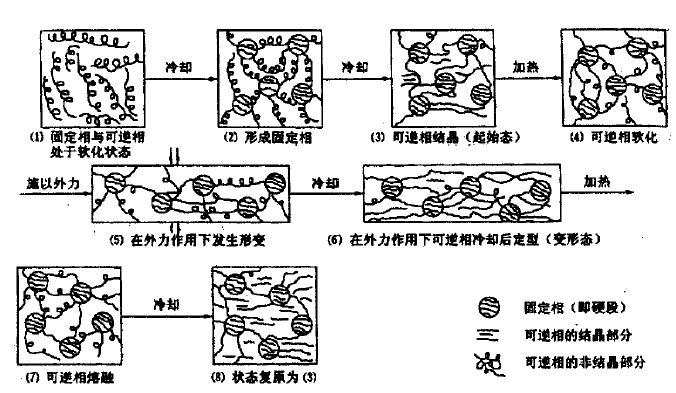
\includegraphics[width=0.75\textwidth]{figures/figure1.png}
	% \caption[这里的文字将会显示在 listoffigure 中]{这里的文字将会显示在正文中}
	\caption{LLMalMorph整体架构。该框架由两大核心模块构成:功能变异模块:从恶意软件源代码文件中提取功能函数,并借助LLM进行修改。变种合成模块:将修改后的函数更新至恶意软件源代码,通过编译项目生成变种文件}\label{fig:4.1}
\end{figure}

Algorithm \ref{alg:Function Transformation Using LLM},专为功能变异模块设计,详细说明了三个子模块 Extractor、Prompt Generator 和 LLM-Based Function Modifier 如何转换恶意软件源代码中的函数。该算法以文件名 $i$、要修改的函数数量 $j$、期望的转换策略 $s$ 以及选定的 $LLM$ 作为输入。接下来,我们将详细描述每个子模块。

\begin{algorithm}[htbp]
	\caption{使用LLM转换函数\label{alg:Function Transformation Using LLM}}
	\KwIn{文件名$i$,需要改变的函数数量 $j$,转换策略 $s$,语言模型 $LLM$}
	\KwOut{转换后的函数集$\hat{F_{s}}=\{\hat{f_{1}^{i}},\hat{f_{2}^{i}}...,\hat{f_{j}^{i}}\}$}

    Headers,globals,functions$\{f_{1}^{i},f_{2}^{i},...,f_{G}^{i}\}\leftarrow extractor(i)$;\\
    初始化转换后的函数集 $\hat{F_{s}}\leftarrow \emptyset$;\\

    \For{$t \gets 1$ \KwTo $j$}{
        $p_{s}||f_{t}^{i} \leftarrow gen\_prompt(s,f_{t}^{i},headers,globals)$;\\
        Transform function: $\hat{f_{t}^{i}} \leftarrow LLM(p_{s}||f_{t}^{i})$;\\
        Update set: $\hat{F_{s}} \leftarrow \hat{F_{s}} \cup \{\hat{f_{t}^{i}}\}$;
    }
    return $\hat{F_{s}}$
\end{algorithm}

\subsection{Extractor子模块}
Extractor 子模块(算法 \ref{alg:Function Transformation Using LLM} 的第 1 行)利用 extractor 子程序,该子程序接收一个源文件并遍历源代码的解析树。它从解析树中提取并存储以下两条辅助信息:全局声明的变量、结构体、编译器指令的列表,并将它们存储于 $globals$ 中;以及所包含头文件的列表,并将它们存储于 $headers$ 中。此类信息对于成功转换至关重要,因为它提供了函数可能使用的全局依赖项的基本上下文。以提示的形式将此上下文提供给 LLM 可确保生成更准确且语法正确的代码。此后,该子程序解析源文件以提取所有函数定义,生成集合$\{f_{1}^{i},f_{2}^{i},...,f_{G}^{i}\}$。

\subsection{Prompt Generator子模块}
算法 \ref{alg:Function Transformation Using LLM} 的第 3−7 行对应于 Prompt Generator 和 LLM Transformation 子模块。第 4 行中的子程序 $gen\_prompt$ 被调用,参数为函数 $f_t^{i}$、转换策略 $s$ 以及提取的 $headers$ 和 $globals$。它将输入代码和策略构造成一个为 LLM 定制的提示 $p_{s}||f_{t}^{i}$。提示的设计详见第 IV-C 节。另请参阅附录 F 了解该子程序中使用的不同类型的提示,以及附录 G 了解一个完整构建的提示及其相应 LLM 响应的示例。

\subsection{LLM Based Function Modifier子模块}
算法 \ref{alg:Function Transformation Using LLM}的第5行将设计好的提示 $p_{s}||f_{t}^{i}$ 提供给选定的$LLM$,并获取转换后的函数。在代码生成过程中,我们使用了LLM的默认推理设置。具体而言,temperature=0.8,top-k=40,top-p=0.9。我们在附录A-A中提供了使用LLM进行代码生成过程的详细描述。

最后,第 6 行将转换后的函数 $f_{t}^{i}$ 追加到输出集合中。一旦所有选定的函数处理完毕,该算法即返回转换后的集合。我们注意到,该算法可以执行多次,以从同一源文件生成函数的多个变体。然而,在本工作中,对于每个选定的恶意软件样本,我们将评估限制在转换后函数的单一版本上。

Algorithm \ref{alg:Malware Variant Generation},在变种合成模块中实现,使用由算法 \ref{alg:Function Transformation Using LLM} 产生的转换后函数集合 $\hat{F_{s}}$、恶意软件项目 $P$ 以及被修改的文件 $i$。它以增量方式生成恶意软件变体,并结合手动调试以确保成功编译。第 1 行初始化恶意软件变体的结果集合 $M_{s}$。该集合包含针对文件 $i$ 使用策略 $s$ 生成的恶意软件变体。尽管我们展示了针对某个特定文件的算法,但当我们处理后续文件时,先前处理过的文件的所有修改都会被保留并向前传递,从而确保恶意软件代码库的累积式转换。该算法的核心功能封装在第 2-10 行中,其中每个转换后的函数被迭代地集成和调试。

\begin{algorithm}[htbp]
	\caption{恶意软件变种生成\label{alg:Malware Variant Generation}}
	\KwIn{恶意软件项目$P$,文件名 $i$,转换后的函数集合 $\{\hat{f_{1}^{i}},\hat{f_{2}^{i}}...,\hat{f_{j}^{i}}\}$}
	\KwOut{编译后的恶意软件变种集合$M_{s}$}
    初始化集合: $M_s \leftarrow \emptyset$;\\
    \For{$t \gets 1$ \KwTo $j$}{
        Extract subset of functions: $\hat{F_{t}} \leftarrow \{\hat{f_{k}^{i}} \in \hat{F_{s}} | 1\leq k\leq t\}$;\\   
        Generate updated file: $\hat{i} \leftarrow merger(i,\hat{F_{t}})$;\\
        \While{$compile(P)$ fails}{
            Debug project $P$ and resolve errors;
        }
        Compile project: $\hat{M_{s}} \leftarrow compile(P)$;\\
        Add compiled malware: $M_{s} \leftarrow M_{s} \cup \hat{M_{s}}$;\\
    }
    return $M_{s}$
\end{algorithm}

\subsection{Merger子模块}
第 3 行首先提取函数子集 $\hat{F_{t}}$,该子集包含函数 1 到 $t$。下一行使用 $merger$ 子程序,用集合 $\hat{F_{t}}$ 更新文件 i。它将更新后的函数集成到文件 $i$ 中,同时保持其余函数不变,并利用在 LLM 使用算法 \ref{alg:Function Transformation Using LLM} 进行代码生成过程中的各种簿记信息。合并后,我们获得包含 $(1...t)$ 个修改后函数的更新文件 $\hat{i}$。$merger$ 子程序的更多细节详见附录 A-B。

\subsection{Compilation and Debugging子模块}
算法 2 的下一步涉及将更新后的文件 $\hat{i}$ 放入恶意软件项目 $P$ 中。第 6–9 行编译更新后的恶意软件项目。如果编译成功,则将生成的恶意软件变体 $\hat{M_{s}}$ 添加到结果集 $M_{s}$ 中。如果编译失败,则进行手动调试以解决错误。

手动调试由一位从事对抗性恶意软件领域和恶意软件分类研究的研究人员执行,这确保了修正的一致性和技术可靠性。调试过程严格解决语法错误、构建和项目配置问题,例如链接外部库或更改语言版本,以及恢复 LLM 遗留的不完整的占位符代码。未对 LLM 生成代码的语义逻辑进行任何更改。代码修正在成功编译修改后的恶意软件源代码的前提下,被刻意限制在最小干预范围内。值得注意的是,调试过程专注于第 $t$ 个函数,因为先前 $(1,...,t − 1)$ 的 LLM 生成函数已经过调试和修正,确保错误不会跨迭代传播。调试完成后,编译成功的恶意软件变体可执行文件被添加到 $M_{s}$ 中。该过程持续增量进行,直到所有函数处理完毕并返回最终的恶意软件变体集合。

\section{B. 代码转换策略}
我们介绍用于通过LLM操作C/C++恶意软件源代码的源代码转换策略。

\subsection{代码优化}
该策略通过提示优化源代码,方法是消除冗余、解决性能瓶颈以及简化代码逻辑,而不改变其核心功能。它涉及使用替代的数据结构和算法,或利用现代库和特定语言特性,例如C++算法头文件中的搜索函数。这些优化可能改变代码的执行和性能特征,有可能降低静态或基于启发式方法的检测率。

\subsection{代码质量与可靠性}
该策略确保生成的代码遵循标准实践,具有改进的错误处理并解决边缘情况。额外的错误处理可防止执行期间的运行时问题,并为代码添加分支,这使恶意软件更加可靠。

\subsection{代码可重用性}
该策略侧重于将大型函数拆分为更小的模块化块。这些较小的函数调用通过改变执行流,有助于掩盖恶意软件的真实行为,这使得依赖涉及控制流执行模式的检测器在实现恶意软件预期相同结果的同时面临更大挑战。

\subsection{代码安全性}
该策略通过遵循安全编码标准来解决潜在的安全漏洞。恶意软件(如勒索软件)严重依赖加密库进行数据加密和解密。此方法提示 LLM 用替代方案替换这些库,修改敏感操作的实现,同时保持恶意软件的核心功能。通过混淆加密行为,检测引擎可能更难以识别该可执行文件为恶意软件。

\subsection{代码混淆}
该策略通过使代码更难以分析和逆向工程来增强恶意软件的规避能力。它包括用无意义的名称重命名函数和变量、添加不必要的控制流结构(例如,跳转、循环)、改变现有控制流以及插入反调试技术。它还定义并调用多余函数,并添加仅在罕见条件下触发的执行路径。这些转换旨在使静态和动态分析复杂化,同时保留恶意软件的核心功能。

\subsection{Windows API 特定转换}
该策略使用提示来识别恶意软件函数内的 Windows API 调用,并引导 LLM 用替代或间接等效的 API 替换它们。它还可能引入包装函数以模糊直接的 API 使用。我们不是使用静态映射,而是利用 LLM 的生成能力来产生多样化的 API 替换,从而增加变异性并避免预定义映射的僵化性和可扩展性问题。尽管功能保持不变,但改变后的 API 模式可能会混淆基于启发式的检测系统(这些系统通常依赖常见的 Windows API 使用模式),从而使恶意软件更难以检测。

\section{C. LLM的快速设计}
在本节中,我们描述用于生成提示的Algorithm \ref{alg:Prompt Construction Subroutine for LLM-based Function Transformation}。我们还介绍了LLM在转换给定函数$f_{t}^{i}$时必须遵循的约束。

它基于给定的转换策略$s$、第$t$个函数$f_{t}^{i}$以及文件$i$的$headers$和$globals$(如算法\ref{alg:Function Transformation Using LLM}中所定义)进行操作。该子程序以调用$system\_prompt$开始,生成$p_{sys}$。这定义了LLM作为专业编码助手的角色,该助手在系统编程以及C、C++和C\#等语言方面拥有专业知识,并确保代码转换是在适当的上下文和能力范围内进行的。随后,$intro\_prompt$通过接收目标函数$f_{t}^{i}$的名称生成$p_{intro}$,并指定必须使用以下预定义策略将提供的函数以及必要的头文件和全局变量转换为变体函数。接下来,使用$strategy\_prompt$和$s$生成转换策略提示$p_{strat}$。这些步骤建立了转换上下文并指导LLM执行所需的修改。

\begin{algorithm}[htbp]
	\caption{基于LLM实现函数转换的快速构造子程序\label{alg:Prompt Construction Subroutine for LLM-based Function Transformation}}
    \SetKwFunction{FFunOne}{$GEN\_PROMPT$}
    \SetKwProg{Fn}{Function}{:}{end}
    \Fn{\FFunOne{$s$, $f_{t}^{i}$, $headers$, $globals$}}{
        $p_{sys} \leftarrow system\_prompt()$;\\
        $p_{intro} \leftarrow intro\_prompt(f_{t}^{i}.name)$;\\
        $p_{strat} \leftarrow strategy\_prompt(s)$;\\
        $p_{pres} \leftarrow preserve\_rules\_prompt(f_{t}^{i}.name)$;\\
        $p_{addit} \leftarrow additional\_prompt(f_{t}^{i}.name)$;\\
        $p_{code} \leftarrow headers \oplus globals \oplus f_{t}^{i}$;\\
        $p_{user} \leftarrow p_{intro} \oplus p_{strat} \oplus p_{preserve} \oplus p_{additional} \oplus p_{code}$;\\
        return $p_{s}||f_{t}^{i} = p_{sys} \oplus p_{user}$;\\
    }
\end{algorithm}

保留提示$p_{pres}$试图确保原始函数和转换后的函数在语义上等价。它明确指示模型不要修改全局定义或自定义元素(变量、对象、常量)以保持功能一致性,从而避免整个代码库中可能出现的语法或语义错误。此外,$p_{addit}$施加严格的准则以保持一致的、符合语法的代码格式并保留函数签名,指示模型仅在单个特定语言的代码块中生成修改后的函数和必要的头文件,以便于解析和后处理。这确保了输出是完整的,不遗留未完成的代码块,并避免重新生成原始函数。

在完成这些步骤后,代码的提示通过组合 $headers$、$globals$ 和函数 $f_{t}^{i}$ 的定义来构建,其中符号$\oplus$代表字符串连接。这使我们能够通过连接第 3−7 行的所有提示来构建总的用户提示 $p_{user}$。然后,通过连接 $p_{sys}$ 和 $p_{user}$ 来构建最终提示 $p_{s}||f_{t}^{i}$。这种结构化的方法确保 LLM 接收到用于转换任务的明确且完整的指令,同时满足所有必要的约束和要求。

\begin{table}[htbp]
	\centering
	\caption{选择的恶意软件样本总结}
	\label{tab:4.1}
	\begin{tabular*}{\textwidth}{@{\extracolsep{\fill}}cccccccc}
		\toprule
		样本 & 语言 & LOC & 文件数量 & 函数数量 & VT率 & HA率 & 类型 \\
		\midrule
		Exeinfector & C++ & 230 & 1 & 4 & 72.009 & 26.67 & 感染型病毒 \\
		Fungus & C++ & 2266 & 15 & 46 & 73.630 & 76 & 通用犯罪软件 \\
		Dexter & C & 2661 & 12 & 61 & 83.020 & 88 & POS木马 \\
		HiddenVNC & C++ & 4959 & 18 & 60 & 76.503 & 75 & HVNC机器人 \\
		Predator & C++ & 4145 & 10 & 102 & 58.797 & 70.333 & 信息窃取 \\
		Prosto-Stealer & C++ & 7436 & 27 & 143 & 62.033 & 72.333 & 信息窃取 \\
        Conti(Cryptor) & C++ & 8031 & 35 & 99 & 65.275 & 79.333 & 勒索软件 \\
        Babuk(Cryptor) & C++ & 3910 & 22 & 62 & 71.759 & 83.667 & 勒索软件 \\
        RedPetya & C++ & 1494 & 5 & 15 & 62.500 & 56.333 & 勒索软件 \\
        RansomWar & C & 1357 & 5 & 13 & 65.728 & 50.333 & 勒索软件 \\
		\bottomrule
	\end{tabular*}
\end{table}
\chapter{评估}
在本节中,我们进行全面评估以回答以下问题:
• RQ1:LLMalMorph 生成的恶意软件变体对广泛使用的防病毒引擎和机器学习分类器的检测具有多强的抗性?其规避能力与最近的对抗性恶意软件生成框架生成的变体相比如何?
• RQ2:不同转换策略间的代码编辑工作量有何差异?这对揭示 LLM 所犯错误类型有何启示?
• RQ3:生成的恶意软件变体是否保留了原始样本的语义和功能?

\section{评估设置}

\subsection{选择样本}
由于最新的恶意软件源代码稀缺,大多数恶意软件研究都集中在可执行文件上。我们检查了公共数据库 [38], [39],发现大多数可用的 Windows 恶意软件源代码是 32 位的,因此我们将研究重点放在 32 位变体上。我们选择了能够编译成可运行可执行文件、并表现出可通过 VirusTotal 或 Hybrid Analysis 检测到的恶意行为(其 AV 检测率≥60\%)的样本。这产生了十个具有不同复杂性和类型的恶意软件候选样本。RansomWar 样本使用 GCC 编译,其余样本使用 Microsoft Visual Studio 2022\footnote{https://visualstudio.microsoft.com/vs/}编译(因为提供了 .sln 文件)。表 II 总结了选定样本的关键细节。对于 Conti 和 Babuk 勒索软件,我们的分析集中在负责加密的加密器组件上。有关样本的详细信息请参见附录 B。

\subsection{评估指标}
我们使用给定的评估指标:防病毒(AV)检测率($R^{\hat{Ms}}$)。我们使用 VirusTotal 评估 AV 检测率,该平台使用来自不同供应商的多个 AV 引擎扫描样本。每个样本可用的检测器数量因可用性而异。令 $D$ 为可用检测器的集合,$\hat{D} \subseteq D$ 为将恶意软件变体标记为恶意的检测器集合。在第 k 次运行时,变体 $\hat{M_{s}}$ 的 AV 检测率 $R^{\hat{M_{s}}}_{k}$ 定义为 $R^{\hat{M_{s}}}_{k} = \frac{|\hat{D}|}{|D|} \times 100$,其中 $|.|$ 表示两个集合的大小。

每个样本将进行$k$次运行,并计算平均检测率$R^{\hat{M_{s}}}=\frac{1}{k} \sum_{i=1}^{k} R_{k}^{\hat{M_{s}}}$。我们在实验中设定 k=3 以解释不同运行间的变异性。我们还使用 Hybrid Analysis,该工具包含静态分析、基于机器学习的分析以及使用不同引擎的多重扫描分析。检测性能以每个恶意软件样本及其变体在 k 次运行上的平均百分比表示。我们使用这两个工具的免费版本,并通过其各自的 API 自动化样本上传、结果检索和后处理。

\subsection{策略导向的机器学习分类器攻击成功率 (ASR)}
攻击成功率 (Attack Success Rate, ASR) 是评估对抗攻击的广泛使用的指标 [20], [40],即生成的恶意软件变体成功逃避目标系统检测的比例。我们针对三种基于机器学习的恶意软件分类器评估 ASR:Malconv [41]、Malgraph [42] 和一个训练好的 ResNet50 恶意软件分类器 [43]。模型细节详见附录 E。令 M 为一个原始恶意软件样本,将我们的策略 s 应用于所有修改文件 $\hat{F} \subseteq F$ 并为 $j$ 个转换函数生成变体 $V_{s}^{M} = \{\hat{M_{1}}, \hat{M_{2}}, ..., \hat{M_{j}}\}$。对于给定的目标分类器 $C$,令 $\hat{V_{s,C}^{M}} = \{ \hat{M} \in V_{s}^{M} : C(\hat{M}) = benign\}$ 为成功逃避 $C$ 的变体子集。则攻击成功率为 $ASR = \frac{|\hat{V_{s,C}^{M}}|}{|V_{s}^{M}|} \times 100$。其中 $|.|$ 表示集合的大小。

\subsection{策略导向的代码编辑工作量 ($W_{s}^{M}$)}
该指标基于需要手动编辑以编译LLM生成代码的总代码行数来比较策略 $s$。值越高表明需要更广泛的手动干预,意味着LLM在该策略下犯了更严重的错误。对于给定的恶意软件 $M$,令 $\hat{F} \subseteq F$ 表示 $F$ 个文件中被修改的文件数量。恶意软件 $M$ 和策略 $s$ 的编辑工作量 $W_s^{M}$ 定义为在文件 $\hat{F}$ 中所有转换后的函数 $\{f_{1}^{i}, f_{2}^{i}... f_{j}^{i}\}$ 上编辑(添加、修改或删除)的总代码行数,计算公式为 $W_{s}^{M}=\sum_{i=1}^{\hat{F}} \sum_{t=1}^{j} L_{edit}(f_{t}^{i})$,其中 $L_{edit}$ 统计函数 $\hat{f_{t}^{i}}$ 被编辑代码的行数。

\subsection{人力投入量化指标 ($H_{s}^{M}$)}
该指标衡量针对每种策略调试和配置恶意软件中转换后函数所需的人力投入。它量化了生成一个成功编译的 PE 文件所需的总工时。对于给定的恶意软件 $M$ 和代码转换策略 $s$,人力投入 $H_{s}^{M}$ 的计算公式为 $H_{s}^{M} = \sum_{i=1}^{\hat{F}} \sum_{t=1}^{j} ManHours(\hat{f_{t}^{i}})$。此处,求和表示在策略 $s$ 下,在修改文件 $\hat{F}$ 中所有转换后的函数 $\{f_{1}^{i},f_{2}^{i}...f_{j}^{i}\}$ 上所花费的总工时。

\subsection{功能保留指标 ($\Phi^{M}$)}
该指标评估了经 LLMalMorph 转换后,恶意软件语义在变体中保留的程度。由于可执行文件固有的复杂性,尚无精确方法能判断恶意软件 $M$ 与其变种 $\hat{M}$ 之间的语义等价性 [44]。因此,文献中遵循的评估方法包括比较恶意软件与其变体之间的 API 调用序列 [22],或通过在沙箱中运行来比较恶意软件及其变体的行为 [20], [23]。

我们采用类似方法,并利用最长公共子序列 (lcs) 算法来比较 $M$ 和 $\hat{M}$ 之间的 API 调用序列。转换后的变体必须保留原始的 API 调用顺序,允许存在不破坏此序列的额外调用。API 调用序列使用专有沙箱收集。归一化的最长公共子序列定义为 $\hat{lcs}(M, \hat{M})= \frac{lcs(M, \hat{M})}{Length(API(M))}$,其中分母是 $M$ 的 API 序列长度。分数范围从 0 到 1,1 表示完全相同的 API 序列。最后,我们计算功能保留率 $\Phi^{M} = \frac{|\hat{M} \in \psi^{\hat{M}}:\hat{lcs}(M,\hat{M}) \geq \delta|}{|\psi^{\hat{M}}|} \times 100$。

此处,$\psi^{\hat{M}}$(总变体集)定义为所有 AV 检测率 $R^{\hat{M_{s}}}$ 低于 $M$ 的基线检测率的恶意软件变体 $\hat{M}$ 的集合。分子代表 $\psi^{\hat{M}}$ 中保留了语义等价性的子集的大小,我们通过考虑归一化的最长公共子序列得分(其值大于预定义阈值 δ)来确定该子集,而 $|\psi^{\hat{M}}|$ 是整个总变体集的大小。我们通过经验分析恶意软件变体和原始样本,选择 $\delta$ 的值为 0.96。我们选取不同样本在离散值集上的恶意软件变体,并将其上传到 Triage Sandbox。我们分析了变体和原始恶意软件样本的报告,以比较行为指标、注册表修改、网络调用等。我们观察到,在某些情况下,行为漂移在分数低于 0.96 时开始出现,而在其他情况下,即使分数略高于该值,功能等价性也得以保持。然而,大多数保留了关键行为的变体得分在 0.96 或以下。因此,我们选择 $\delta = 0.96$ 作为上限,以确保被接受的变体在 API 序列和执行行为上保持高度相似性。

\section{模型选择}
虽然 LLMalMorph 可以利用任何 LLM 生成恶意软件变体,但我们选择 Codestral-22B [8] 作为我们的主要 LLM。我们精心设计的提示包含许多需要遵循的约束和指示。我们观察到 Codestral 模型能够比其他模型更精确地遵循这些特定指令来变异函数。此外,Codestral 为我们的用例提供了一组均衡的特性——220 亿参数、12 GB 模型大小和 32K 上下文窗口——并且与具有更高硬件要求的模型相比,它在长距离仓库级代码补全任务上具有卓越性能 [4], [9]。

\chapter{相关工作}

恶意软件变体生成的研究已探索多种方法。大量工作聚焦于全局或局部修改恶意软件的二进制代码,通过在特定位置注入或追加字节而不改变其行为来保持原始功能[18], [45]–[49]。另一种方法涉及二进制多样化技术以全局改变恶意软件的二进制文件[20], [50]。此外,利用贪婪算法、基于梯度的优化、生成模型和启发式技术添加无关函数来操控API调用,已成为重要研究领域[23], [51]–[53]。另有方法通过修改底层汇编代码或使用搜索算法/基于学习的优化在特征空间内改变控制流图[22], [29]。直接扰动恶意软件代码空间的研究虽较少探索,但包括注入汇编代码以调用外部DLL来触发额外API而不改变控制流[54]。Murali等人[21]提出的方法操作LLVM生成的中间表示,通过策略性转换直接修改系统调用有向图,随后重新生成恶意软件可执行文件。Choi等人[19]采用名为AMVG的自适应框架,通过解析源代码并运用遗传算法生成恶意软件变体。他们在部分Python样本和良性C程序上展示了简单转换的结果,但仅限于复杂度较低的案例。
\chapter{结论和未来工作}
本研究中,我们提出了LLMalMorph框架——该框架利用LLM通过工程化提示和代码转换策略生成恶意软件变体。采用6种策略生成618个变体,证明了特定转换能降低AV检测率,并在机器学习分类器上具有显著攻击成功率。同时观察到复杂恶意软件常需大量调试以维持功能,这凸显了人工监督的必要性、提示设计的谨慎性,以及当前LLM在恶意软件源代码转换中的局限性。

尽管本研究展示了LLM生成规避性恶意软件变体的潜力,仍存在若干局限。我们的实现可通过增强提取器与合并器子模块扩展到其他语言。未来计划拓展至LLM二进制恶意软件转换,并利用LLM代理提升自动化水平。此外,旨在通过分离恶意软件相关模式改进函数选择机制,并在API序列之外开发更鲁棒的语义保留评估指标。
\chapter{致谢}

本研究由思科研究院(Cisco Research)提供支持。我们衷心感谢思科在本研究全程提供的资金支持与宝贵指导。本文表述的任何结论、观点或建议均代表作者立场,并不必然代表资助方的立场。


\chapter{附录A}

\begin{table}[htb]
	\centering
	\caption{修改的函数选择标准}
	\label{tab:function_selection_criteria_for_modification}
    \begin{tabularx}{\textwidth}{@{} 
    >{\RaggedRight}p{0.5\textwidth} 
    >{\RaggedRight}p{0.5\textwidth} 
    @{}}
		\toprule
		函数数量 & 修改率 \\
		\midrule
		\textless 10  & 100\% \\
		10 - 20 & 60\% \\
        20 - 40  & 30\% \\
		40 - 70 & 20\% \\
        \textgreater 70  & 15\% \\
		\bottomrule
	\end{tabularx}
\end{table}


\chapter{附录B-详细的恶意软件描述}
我们提供了为进行实验而选择的每个恶意软件样本的详细描述。我们还通过Triage Sandbox运行了所有样本,以从沙箱报告中了解它们的行为。对于两个样本,沙箱未提供有用信息,但我们添加了其余样本的描述,我们从沙箱中获得这些样本的信息。

Exeinfector

Exeinfector在相关的GitHub仓库[38]中被归类为感染型,并且VirusTotal为其标记了诸如持久化、长时间休眠、反调试(以及用户输入检测等行为。Triage沙箱报告显示了恶意活动,包括添加持久化运行项、修改注册表、在system32目录中释放文件以及执行系统语言发现。

Fungus

Fungus在相关的GitHub仓库[38]中被归类为通用犯罪软件,是一种复杂的多文件C++恶意软件。VirusTotal将其与ircbot和autorun7等家族标签相关联。它具有反沙箱技术、基于USB的传播、服务器通信、防火墙规避以及键盘记录能力。Triage报告指出其活动包括设置自动启动、加载DLL、执行释放的文件、修改注册表、执行系统语言和位置发现以及可疑地使用Windows API调用。

Dexter
Dexter是一种销售点木马,被识别为针对运行Microsoft Windows的POS机的恶意软件[55]。它于2012年被发现,以从POS机窃取信用卡和借记卡信息、将收集的数据发送到预定服务器以及表现出类僵尸程序行为而闻名[56]。VirusTotal将Dexter分类为木马、勒索软件和下载器,带有poxters和dexter等家族标签。Triage报告指出它会删除自身、崩溃、通过修改注册表添加运行项以实现持久化、执行系统语言发现以及使用可疑的Windows API函数,如“AdjustPrivilegeToken”、“WriteProcessMemory”和“EnumerateProcess”

HiddenVNC Bot

HiddenVNC,根据其源代码readme文件开发于2021年,是一种多文件的复杂C++恶意软件。VirusTotal将其分类为木马和银行木马,将其与tinukebot、tinynuke和tinuke等家族标签相关联,表明它可能是以开后门、窃取信息和下载恶意文件而闻名的Tinynuke木马僵尸程序的一个实现[57]。该readme将其描述为一个隐藏虚拟网络计算工具,它创建一个“隐藏桌面”,允许攻击者在用户不知情的情况下控制目标机器。其功能包括控制多台机器、启动应用程序(例如浏览器、PowerShell)以及在隐藏桌面上执行远程命令。它生成两个可执行文件;我们使用VirusTotal检测率为76.503\%的Client.exe,因为它比Server.exe(15.277\%)更具恶意性。

Predator

Predator,也称为Predator the Thief,于2018年中首次被发现[58]。该样本是一种复杂的C++信息窃取木马,从其受感染主机窃取广泛的数据,例如系统信息、存储的浏览器密码、cookie、表单数据,甚至加密货币钱包地址[58]。它还能捕获网络摄像头照片、记录击键、从应用程序(例如VPN、FTP、游戏客户端)提取凭证,并收集剪贴板内容和加密货币钱包文件[59]。VirusTotal将其归类为木马,并与窃取器、adwarex和fragtor等家族标签相关联。Triage沙箱报告向我们显示,它读取FTP客户端存储的数据文件、读取Web浏览器的用户/配置文件数据、从不安全的文件中窃取凭证、访问加密货币钱包并可能执行凭据收集。

Prosto

Prosto,也称为ProstoStealer,同样是一种信息窃取木马,但比Predator样本大得多且复杂得多,并且是用C++编写的。它利用受害机器窃取有价值且有用的信息,如登录信息、凭证、密码和直接文件。所有细节都存储在由攻击者控制的服务器中,以便后续用于诈骗和欺诈活动[60]。VirusTotal将此样本分类为木马、病毒和间谍软件,并用fragtor和convagent等家族标签进行标记。该样本的Triage沙箱报告告诉我们,它会检查计算机位置设置、读取Web浏览器的用户数据、修改Internet Explorer设置,并且还有可疑地使用“FindShellTrayWindow”、“SetWindowsHookEx”、“WriteProcessMemory”等方法。

Conti

Conti勒索软件于2019年末出现[61]。这是一种极其复杂的恶意软件,包含不同的活动部件,拥有超过8000行用C++编写的代码。在我们的实验中,我们使用该样本的cryptor可执行文件。它采用双重勒索策略,在窃取数据的同时加密文件,以迫使受害者支付赎金。它以其快速的加密速度和针对医疗保健等关键行业而闻名[61]。VirusTotal将该可执行文件分类为木马和勒索软件,并将其与conti和adwarex等家族标签相关联。

Babuk

Babuk,也称为Babyk,是一种复杂的勒索软件,于2021年初被发现[62],针对多个平台,如Windows、适用于Linux的ARM以及VMware ESXI环境,并使用椭圆曲线算法构建加密密钥[63]。该勒索软件用C++编写,约4000行代码,极其复杂,针对多个国家和地区的医疗保健、塑料、运输、电子和农业等行业[62]。我们在实验中使用了该勒索软件的加密模块,并使用了生成的“.bin”格式可执行文件。VirusTotal将其归类为勒索软件和木马,并用babuk、babyk和epack等家族标签进行标记。Triage报告向我们显示,它是一种babuk加密器并属于babuk家族,会删除自身的卷影副本、重命名多个文件并添加文件扩展名、枚举已连接的驱动器和物理存储设备、与卷影副本交互,并且还有各种可疑的Windows API使用。

RedPetya Ransomware

RedPetya属于Petya家族加密恶意软件,于2016年首次被发现[64]。它采用引导锁式加密,在感染受害者后覆盖系统的主引导记录并强制重启;此时不是加载Windows,而是显示一个虚假屏幕,同时恶意软件使用加密算法在磁盘上秘密加密NTFS主文件表[65]。我们使用了其源代码的一个开源版本,该版本用C++编写,约1500行代码,使用OpenSSL进行加密,是对RedPetya恶意软件的完全重写。VirusTotal将此样本分类为木马和勒索软件,并给出petya、heur3和diskcoder等家族标签。Triage报告还显示它具有持久性,是一个引导区病毒,并且会写入主引导记录。它还显示可疑地使用Windows API,如“EnumeratesProcesses”、“AdjustPrivilegeToken”。

RansomWar

该样本是一种相对简单的勒索软件,用C语言编写,共1377行代码,使用河豚加密算法加密文件,并且代码中内置了邮件发送机制。VirusTotal将其归类为木马、勒索软件,并给出barys、ransomware等家族标签。从Triage沙箱中,我们得知它会枚举已连接的驱动器并在System32目录中释放文件。



\chapter{附录C-用于LLM修改的文件及恶意软件函数选择数量}

本节阐述我们从每个恶意软件样本中选择待修改函数数量的方法。表~\ref{tab:4.1}虽概述了各恶意软件样本的函数总量,但我们的选择过程需经严格筛选以确保修改的有效性。我们排除了属于外部库(如加密库和头文件)的文件,仅聚焦于包含自定义恶意软件代码的文件,并仅考虑按算法~\ref{alg:Function Transformation Using LLM}顺序修改全局函数。

鉴于不同恶意软件样本的函数数量存在差异,我们采用系统化策略:对函数较少的样本修改更大比例,而对函数数量显著的样本则修改较小比例。该方法在保证充分修改覆盖率与LLMalMorph所需可控人工调试工作量之间取得了平衡。

应用该方法,我们选取并修改了如下函数:
\begin{table}[htb]
	\centering
	\caption{修改的函数选择标准}
	\label{tab:function_selection_criteria_for_modification}
    \begin{tabularx}{\textwidth}{@{} 
    >{\RaggedRight}p{0.5\textwidth} 
    >{\RaggedRight}p{0.5\textwidth} 
    @{}}
		\toprule
		函数数量 & 修改率 \\
		\midrule
		\textless 10  & 100\% \\
		10 - 20 & 60\% \\
        20 - 40  & 30\% \\
		40 - 70 & 20\% \\
        \textgreater 70  & 15\% \\
		\bottomrule
	\end{tabularx}
\end{table}

应用此方法,我们选择并修改了以下函数:
\begin{table}[htb]
	\centering
	\caption{每个恶意软件样本的函数选择}
	\label{tab:function_selection_for_each_malware_sample}
    \begin{tabularx}{\textwidth}{@{} 
    >{\RaggedRight}p{0.25\textwidth} 
    >{\centering}p{0.25\textwidth} 
    >{\centering}p{0.25\textwidth} 
    >{\RaggedRight}p{0.25\textwidth} 
    @{}}
		\toprule
		恶意软件样本 & 总共选择的函数 & 修改的函数 & 修改率 \\
		\midrule
		Exeinfector & 4 & 4 & 100\% \\
		Fungus & 46 & 9 & 20\% \\
        Dexter & 61 & 12 & 20\% \\
		HiddenVNC bot & 60 & 12 & 20\% \\
        Predator & 30 & 9 & 30\% \\
        Prostostealer & 70 & 14 & 20\% \\
		Conti ransomware & 93 & 14 & 15\% \\
        Babuk ransomware & 35 & 11 & 30\% \\
		RedPetya & 15 & 9 & 60\% \\
        ransomware & 9 & 9 & 100\% \\
		\bottomrule
	\end{tabularx}
\end{table}

在必要处我们进行向上取整。对于RansomWar样本,我们最初尝试修改包含4个函数的"blowfish.c"文件未能成功,这源于LLM即使在纠错机制下仍存在生成函数变体的限制。因此,我们将修改转向包含9个函数的"RansomWar.c"文件。由于该文件属于函数数量少于10的样本类别,我们修改了其全部函数。总体而言,这种结构化方法使我们能在保持一致性的同时,确保不会在函数数量庞大的样本(例如Conti勒索软件)中修改过多函数——这考虑到LLMalMorph所需的人工调试需求。
\chapter{附录D-额外恶意软件检测率分析}
VirusTotal的Dexter分析

如图2a中Dexter的第三子图所示,优化策略检测率持续下降,在六次函数修改后稳定在均值附近。当修改文件"injectSection"(负责进程代码注入和资源管理)中的第二个函数后,"复用性"策略检测率骤降至67.847\%。尽管该函数初始导致检测率下降,但随后回升至74.537\%。其余策略检测率则始终接近整体平均值。

VirusTotal的Prosto分析

如图2a中Prosto窃取器样本的第六子图所示,检测率波动显著:复用性策略在第4至第6次修改间急剧下降,优化策略则在第10至第11次修改间出现陡降。优化、Windows及安全策略均呈下降趋势,其中优化策略最低达52.738\%,较基线62.033\%降低9.295\%。LLM采用替代性Windows API函数进行Base64编码和HTTP连接管理可能导致此下降。

VirusTotal的Babuk分析

如图2a中Babuk勒索软件样本的第八子图所示,优化策略在第二个函数修改起始处出现显著下降,检测率达64.861\%,较基线71.759\%降低近7\%。该变体在此策略的分数微升但仍低于基线检测率。除"复用性"外所有策略均呈现类似趋势,但检测率下降幅度不大。

Hybrid Analysis的Predator分析

如图2b中Predator窃取器样本的第五子图所示,除Predator子图中少量偏移数据点外,多数变体呈现极小波动。值得注意的是,优化策略检测率略低于其他变体。

Hybrid Analysis的Prosto分析

如图2b中Prosto窃取器样本的第六子图所示,多数变体聚集在72.33\%的基线检测率附近且偏差较小。未发现任何特定策略变体呈现显著低于基线的检测率。

Hybrid Analysis的Conti分析

在Conti勒索软件的分析图中,71.568\%的平均检测率较基线79.333\%低约8\%。优化策略在第5至第6个函数修改处出现急剧下降,后续函数检测率维持在65\%左右。此外,质量策略的检测率同样呈现下降趋势。
\chapter{机器学习模型与阈值详情}

本节详述机器学习模型的具体架构。Malconv主要采用卷积神经网络设计,通过将恶意软件作为原始字节流处理进行分类。ResNet50分类器底层使用原始ResNet50模型[66],该模型首先将恶意软件转换为灰度图像,再利用图像进行分类。而Malgraph模型不直接使用图像/可执行文件,它是一种分层图恶意软件分类器,采用两个基于图神经网络(GNN)的编码层:函数内层将单个函数的控制流图(CFG)编码为向量,函数间层则利用前层生成的向量及外部函数,对函数调用图(FCG)表征进行编码以学习全局程序表示。最终预测层对此嵌入向量应用多层感知机(MLP)计算恶意概率。

对于Malconv和MalGraph,我们采用文献[22]提供的现成实现,该模型基于文献[42]所引入的数据集训练——该数据集包含210,251个Windows可执行文件(101,641个恶意软件和108,610个正常软件),涵盖848个恶意软件家族。数据集构成与模型性能的补充细节详见[22]。针对ResNet50,我们采用预训练的ImageNet模型,基于文献[43]最新提出的恶意软件图像表征进行微调,该数据集包含恶意软件样本(2024年3月、4月、5月、7月和8月从MalwareBazaar\footnote{https://bazaar.abuse.ch/}收集)及对应正常软件。训练数据包含7,312个恶意软件实例和14,338个正常软件实例,恶意软件与正常软件比例为0.5:1。此训练分类器的性能在独立测试集上评估,该测试集包含9月恶意软件(同样采集自Malwarebazaar)和正常软件样本,恶意软件与正常软件比例为0.44:1(1,337个恶意软件和3,020个正常软件)。分类器在此测试集达到85\%准确率和85\% F1分数,更多细节参见[43]。

对于所有三个分类器,我们采用文献[22]设定的0.1\%误报率(FPR)阈值。恶意软件检测中需要低误报率以减少对良性文件的误判,但这也提高了决策阈值,可能导致更高的攻击成功率。此权衡关系已在先前研究[22]中被指出。针对Malconv和MalGraph,文献[22]提供的现成实现已包含0.1\% FPR阈值。对于微调后的ResNet50模型,我们通过选择良性测试集(仅用于阈值校准而非评估)上恶意软件概率的99.9百分位点计算等效阈值。在此模型特定阈值下,Malconv和ResNet50均未标记10个原始恶意软件样本,仅Malgraph标记了Fungus、Dexter、Conti和Babuk。故而我们将对抗评估集中于这四个样本变体。
\chapter{所有提示词}


我们提供通过算法~\ref{alg:Prompt Construction Subroutine for LLM-based Function Transformation}所述LLM修改LLMalMorph函数所使用的全部提示词:
\section{A. 系统提示词}
System Prompt: You are an intelligent coding assistant who is expert in writing, editing, refactoring and debugging code. You listen to exact instructions and specialize in systems programming and use of C, C++ and C\# languages with Windows platforms

\section{B. 介绍提示词}
Below this prompt you are provided headers, global variables, class and struct definitions and self.num\_functions global function definition(s) from a self.language\_name source code file. The parameters of the functions also have specific types. As an intelligent coding assistant, GENERATE one VARIANT of each of these functions: ***’, ’.join([func\_name for func\_name in self.function\_names])*** following these instructions:

\section{C. 代码转换策略提示词}
如第四-B小节所述,我们开发了六种代码转换策略。各策略具体提示词如下:

\subsection{代码优化}
1. Remove code redundancies.

2. Identify performance bottlenecks and fix them.

3. Simplify the code’s logic or structure and optimize data structures and algorithms if applicable.

4. Use language-specific features or modern libraries if applicable.

\subsection{代码质量与可靠性}
1. Check error handling and edge cases.

2. Follow coding practices and style guidelines.

3. Add proper documentation to classes and functions, and comments for complex parts.

\subsection{代码复用性}
Make the code reusable by dividing supplied functions into smaller function blocks if and where applicable. The smaller functions should be called inside the respective supplied functions as needed.

\subsection{代码安全性}
1.Identify security vulnerabilities and fix them.

2.If the function you are modifying contains cryptographic operations,change the cryptographic library used for those operations.If no cryptographic operations are present,no changes are necessary.

3.Follow secure coding standards and guidelines.

\subsection{代码混淆}
1. Change the given function’s and LOCAL variable’s names to meaningless, hard-to-understand strings which are not real words. DO NOT redefine or rename global variables (given to you) and names of functions that are called inside the given function ( might be defined elsewhere ) under any circumstances. However if the given function name is any of ‘main‘, ‘wmain‘, ‘WinMain‘, ‘wWinMain‘, ‘DllMain‘, ‘\_tWinMain‘, ‘\_tmain‘ do not change it’s name, only change the local variable’s names inside the function.

2. Add unnecessary jump instructions, loops, and conditional statements inside the functions.

3. Add unnecessary functions and call those functions inside the original functions.

4. Add anti-debugging techniques to the code.

5. If there are loops/conditional statements in the code change them to their equivalent alternatives and make them more difficult to follow.

6. Incorporate code to the variants that activates under very rare and obscure cases without altering core functionality, making the rare code hard to detect during testing.

\subsection{WindowsAPI专用转换}
1. Identify all Windows API function calls in the given functions.

2. If there are such function calls, replace each identified Windows API function call with an alternative Windows API function call or sequence of calls that achieves the same task.

3. If applicable, use indirect methods or wrappers around the Windows API calls to achieve the same functionality.

4. Ensure that the functionality remains the same after the replacement.

\section{D. 保留规则提示词}
REMEMBER, the generated code MUST MAINTAIN the same FUNCTIONALITY as the original code. Keep the usage of globally declared variables as it is. Modify ONLY the self.num\_functions free/global function(s) named ***’, ’.join([func\_name for func\_name in self.function\_names])***. If you find any custom functions/custom structure/class objects/custom types/custom variables that are used inside the given self.num\_functions function(s) but not in the provided code snippet, you can safely assume that these are defined elsewhere and you should use them in your generated code as it is. DO NOT modify the names of these and do not redefine them.

\section{E. 附加约束}
These CRUCIAL instructions below MUST ALWAYS BE FOLLOWED while generating variants:
1. You MUST NOT regenerate the extra information I provided to you such as headers, global variables, structs and classes for context.

2. If you modify the functions ***’, ’.join([func\_name for func\_name in self.function\_names])***, you MUST NOT regenerate the original code. But if a function cannot be changed, then include the original code. 

3. ONLY generate the function variants and any new headers/libraries you used.

4. You MUST NOT generate any extra natural language messages/comments.

5. You MUST Generate all the modified functions within a single ‘‘‘self.language\_name ‘‘‘ tag. For example your response should look like this for one generatedfunction named ‘int func(int a)‘: f"{example\_code}" Remember, if you have generated multiple functions, you should include all of them within the same ‘‘‘self.language\_name ‘‘‘ tag.

6. Use the global variables as they are inside your generated functions and do not change/redeclare the global variables.

7. Always complete the function that you generate. Make sure to fill up the function body with the appropriate code. DO NOT leave any function incomplete.

上述提示词使用的"example\_code":

’c’:‘‘‘self.language\_name
 \#include<stdio.h>
 intfunc(inta) \{ printf("\%d",a);returna+1; \}
‘‘‘
’cpp’:‘‘‘self.language\_name
 \#include<iostream>
 intfunc(inta) \{ cout<<a<<endl;return a +1; \}
‘‘‘
\backmatter

% 结论
%%%
% BIThesis 研究生学位论文模板 The BIThesis Template for Graduate Thesis
% This file has no copyright assigned and is placed in the Public Domain.
%%

\begin{conclusion}

本文采用……。{\color{blue}(结论作为学位论文正文的最后部分单独排写,但不加章号。结论是对整个论文主要结果的总结。在结论中应明确指出本研究的创新点,对其应用前景和社会、经济价值等加以预测和评价,并指出今后进一步在本研究方向进行研究工作的展望与设想。结论部分的撰写应简明扼要,突出创新性。)}

\end{conclusion}

% 参考文献
%%
% BIThesis 研究生学位论文模板 The BIThesis Template for Graduate Thesis
% This file has no copyright assigned and is placed in the Public Domain.
%%

%
% 如无特殊需要,本页面无需更改。
%
% **注意:如果发现渲染出来的文献编号不正确,请同时使用以下两个方式解决:**
% 1. 清除缓存后重新编译(比如使用 `latexmk -c`)。
% 2. 请确保无编译错误。


\begin{bibprint}
  \printbibliography[heading=none,notcategory=mypub,resetnumbers=true]
\end{bibprint}


% 附录
%%%
% BIThesis 研究生学位论文模板 The BIThesis Template for Graduate Thesis
% This file has no copyright assigned and is placed in the Public Domain.
%%

\begin{appendices}
\chapter{不同子程序的细节}
\section{A. 关于基于LLM的代码生成的细节}
如算法1所述,我们将提示连同函数和相关信息传递给LLM,以生成修改后的代码。LLM处理该提示并产生响应,我们解析该响应以提取生成的代码。在生成代码时,我们遇到了两个关键挑战性案例:

• LLM偶尔未能以期望的格式生成代码。
• LLM有时会描述给定函数的机制,而不是生成任何代码。

在第二种情况中,模型要么提供了对输入函数的详细解释,要么基于提供的上下文将该函数识别为潜在恶意并生成了对给定代码的分析。为了解决这些挑战,我们实现了一个重试机制。当任一情况发生时,我们使用不同的随机种子最多提示LLM五次。如果LLM仍然未能生成可用的代码,我们则回退到原始函数并继续进行解析代码的下一步。由于我们提示模型以特定格式生成代码,因此我们可以从生成的响应中解析代码,保存生成的代码,并记录有用的信息以供我们的指标计算,例如生成的代码行数、生成代码所需的时间、生成代码的路径等。我们在算法~\ref{alg:Malware Variant Generation}后续的合并阶段利用了这些信息。

\section{B. 关于“merger”子程序的细节}
该子程序仔细追踪哪些函数需要更新、哪些保持不变,在整个过程中保持两者之间的明确区分。它保留源文件中的原始头声明和全局变量,以保持项目范围内的一致性。这种方法防止了文件内部或延伸到其他文件中可能出现的依赖关系的潜在破坏。此外,我们指示LLM避免声明任何全局变量,并仅依靠创建和使用函数内部的局部变量。这确保了模块化并防止了意外的副作用。在转换后的函数被拆分为子函数的情况下,“merger”子程序有条不紊地定义它们的原型,将这些子函数放置在文件的开头,并整合了修改后的原始函数,该函数现在调用这些子函数。
通过遵循这些准则,“merger”子程序确保了转换后函数的集成是健壮和结构化的,并最大程度地降低了在代码库中引入不一致性的风险。


\chapter{详细的恶意软件描述}
我们提供了为进行实验而选择的每个恶意软件样本的详细描述。我们还通过Triage Sandbox运行了所有样本,以从沙箱报告中了解它们的行为。对于两个样本,沙箱未提供有用信息,但我们添加了其余样本的描述,我们从沙箱中获得这些样本的信息。

Exeinfector

Exeinfector在相关的GitHub仓库[38]中被归类为感染型,并且VirusTotal为其标记了诸如持久化、长时间休眠、反调试(以及用户输入检测等行为。Triage沙箱报告显示了恶意活动,包括添加持久化运行项、修改注册表、在system32目录中释放文件以及执行系统语言发现。

Fungus

Fungus在相关的GitHub仓库[38]中被归类为通用犯罪软件,是一种复杂的多文件C++恶意软件。VirusTotal将其与ircbot和autorun7等家族标签相关联。它具有反沙箱技术、基于USB的传播、服务器通信、防火墙规避以及键盘记录能力。Triage报告指出其活动包括设置自动启动、加载DLL、执行释放的文件、修改注册表、执行系统语言和位置发现以及可疑地使用Windows API调用。

Dexter
Dexter是一种销售点木马,被识别为针对运行Microsoft Windows的POS机的恶意软件[55]。它于2012年被发现,以从POS机窃取信用卡和借记卡信息、将收集的数据发送到预定服务器以及表现出类僵尸程序行为而闻名[56]。VirusTotal将Dexter分类为木马、勒索软件和下载器,带有poxters和dexter等家族标签。Triage报告指出它会删除自身、崩溃、通过修改注册表添加运行项以实现持久化、执行系统语言发现以及使用可疑的Windows API函数,如“AdjustPrivilegeToken”、“WriteProcessMemory”和“EnumerateProcess”

HiddenVNC Bot

HiddenVNC,根据其源代码readme文件开发于2021年,是一种多文件的复杂C++恶意软件。VirusTotal将其分类为木马和银行木马,将其与tinukebot、tinynuke和tinuke等家族标签相关联,表明它可能是以开后门、窃取信息和下载恶意文件而闻名的Tinynuke木马僵尸程序的一个实现[57]。该readme将其描述为一个隐藏虚拟网络计算工具,它创建一个“隐藏桌面”,允许攻击者在用户不知情的情况下控制目标机器。其功能包括控制多台机器、启动应用程序(例如浏览器、PowerShell)以及在隐藏桌面上执行远程命令。它生成两个可执行文件;我们使用VirusTotal检测率为76.503\%的Client.exe,因为它比Server.exe(15.277\%)更具恶意性。

Predator

Predator,也称为Predator the Thief,于2018年中首次被发现[58]。该样本是一种复杂的C++信息窃取木马,从其受感染主机窃取广泛的数据,例如系统信息、存储的浏览器密码、cookie、表单数据,甚至加密货币钱包地址[58]。它还能捕获网络摄像头照片、记录击键、从应用程序(例如VPN、FTP、游戏客户端)提取凭证,并收集剪贴板内容和加密货币钱包文件[59]。VirusTotal将其归类为木马,并与窃取器、adwarex和fragtor等家族标签相关联。Triage沙箱报告向我们显示,它读取FTP客户端存储的数据文件、读取Web浏览器的用户/配置文件数据、从不安全的文件中窃取凭证、访问加密货币钱包并可能执行凭据收集。

Prosto

Prosto,也称为ProstoStealer,同样是一种信息窃取木马,但比Predator样本大得多且复杂得多,并且是用C++编写的。它利用受害机器窃取有价值且有用的信息,如登录信息、凭证、密码和直接文件。所有细节都存储在由攻击者控制的服务器中,以便后续用于诈骗和欺诈活动[60]。VirusTotal将此样本分类为木马、病毒和间谍软件,并用fragtor和convagent等家族标签进行标记。该样本的Triage沙箱报告告诉我们,它会检查计算机位置设置、读取Web浏览器的用户数据、修改Internet Explorer设置,并且还有可疑地使用“FindShellTrayWindow”、“SetWindowsHookEx”、“WriteProcessMemory”等方法。

Conti

Conti勒索软件于2019年末出现[61]。这是一种极其复杂的恶意软件,包含不同的活动部件,拥有超过8000行用C++编写的代码。在我们的实验中,我们使用该样本的cryptor可执行文件。它采用双重勒索策略,在窃取数据的同时加密文件,以迫使受害者支付赎金。它以其快速的加密速度和针对医疗保健等关键行业而闻名[61]。VirusTotal将该可执行文件分类为木马和勒索软件,并将其与conti和adwarex等家族标签相关联。

Babuk

Babuk,也称为Babyk,是一种复杂的勒索软件,于2021年初被发现[62],针对多个平台,如Windows、适用于Linux的ARM以及VMware ESXI环境,并使用椭圆曲线算法构建加密密钥[63]。该勒索软件用C++编写,约4000行代码,极其复杂,针对多个国家和地区的医疗保健、塑料、运输、电子和农业等行业[62]。我们在实验中使用了该勒索软件的加密模块,并使用了生成的“.bin”格式可执行文件。VirusTotal将其归类为勒索软件和木马,并用babuk、babyk和epack等家族标签进行标记。Triage报告向我们显示,它是一种babuk加密器并属于babuk家族,会删除自身的卷影副本、重命名多个文件并添加文件扩展名、枚举已连接的驱动器和物理存储设备、与卷影副本交互,并且还有各种可疑的Windows API使用。

RedPetya Ransomware

RedPetya属于Petya家族加密恶意软件,于2016年首次被发现[64]。它采用引导锁式加密,在感染受害者后覆盖系统的主引导记录并强制重启;此时不是加载Windows,而是显示一个虚假屏幕,同时恶意软件使用加密算法在磁盘上秘密加密NTFS主文件表[65]。我们使用了其源代码的一个开源版本,该版本用C++编写,约1500行代码,使用OpenSSL进行加密,是对RedPetya恶意软件的完全重写。VirusTotal将此样本分类为木马和勒索软件,并给出petya、heur3和diskcoder等家族标签。Triage报告还显示它具有持久性,是一个引导区病毒,并且会写入主引导记录。它还显示可疑地使用Windows API,如“EnumeratesProcesses”、“AdjustPrivilegeToken”。

RansomWar

该样本是一种相对简单的勒索软件,用C语言编写,共1377行代码,使用河豚加密算法加密文件,并且代码中内置了邮件发送机制。VirusTotal将其归类为木马、勒索软件,并给出barys、ransomware等家族标签。从Triage沙箱中,我们得知它会枚举已连接的驱动器并在System32目录中释放文件。



\chapter{用于LLM修改的文件及恶意软件函数选择数量}

本节阐述我们从每个恶意软件样本中选择待修改函数数量的方法。表~\ref{tab:4.1}虽概述了各恶意软件样本的函数总量,但我们的选择过程需经严格筛选以确保修改的有效性。我们排除了属于外部库(如加密库和头文件)的文件,仅聚焦于包含自定义恶意软件代码的文件,并仅考虑按算法~\ref{alg:Function Transformation Using LLM}顺序修改全局函数。

鉴于不同恶意软件样本的函数数量存在差异,我们采用系统化策略:对函数较少的样本修改更大比例,而对函数数量显著的样本则修改较小比例。该方法在保证充分修改覆盖率与LLMalMorph所需可控人工调试工作量之间取得了平衡。

应用该方法,我们选取并修改了如下函数:
\begin{table}[htb]
	\centering
	\caption{修改的函数选择标准}
	\label{tab:function_selection_criteria_for_modification}
    \begin{tabularx}{\textwidth}{@{} 
    >{\RaggedRight}p{0.5\textwidth} 
    >{\RaggedRight}p{0.5\textwidth} 
    @{}}
		\toprule
		函数数量 & 修改率 \\
		\midrule
		\textless 10  & 100\% \\
		10 - 20 & 60\% \\
        20 - 40  & 30\% \\
		40 - 70 & 20\% \\
        \textgreater 70  & 15\% \\
		\bottomrule
	\end{tabularx}
\end{table}

应用此方法,我们选择并修改了以下函数:
\begin{table}[htb]
	\centering
	\caption{每个恶意软件样本的函数选择}
	\label{tab:function_selection_for_each_malware_sample}
    \begin{tabularx}{\textwidth}{@{} 
    >{\RaggedRight}p{0.25\textwidth} 
    >{\centering}p{0.25\textwidth} 
    >{\centering}p{0.25\textwidth} 
    >{\RaggedRight}p{0.25\textwidth} 
    @{}}
		\toprule
		恶意软件样本 & 总共选择的函数 & 修改的函数 & 修改率 \\
		\midrule
		Exeinfector & 4 & 4 & 100\% \\
		Fungus & 46 & 9 & 20\% \\
        Dexter & 61 & 12 & 20\% \\
		HiddenVNC bot & 60 & 12 & 20\% \\
        Predator & 30 & 9 & 30\% \\
        Prostostealer & 70 & 14 & 20\% \\
		Conti ransomware & 93 & 14 & 15\% \\
        Babuk ransomware & 35 & 11 & 30\% \\
		RedPetya & 15 & 9 & 60\% \\
        ransomware & 9 & 9 & 100\% \\
		\bottomrule
	\end{tabularx}
\end{table}

在必要处我们进行向上取整。对于RansomWar样本,我们最初尝试修改包含4个函数的"blowfish.c"文件未能成功,这源于LLM即使在纠错机制下仍存在生成函数变体的限制。因此,我们将修改转向包含9个函数的"RansomWar.c"文件。由于该文件属于函数数量少于10的样本类别,我们修改了其全部函数。总体而言,这种结构化方法使我们能在保持一致性的同时,确保不会在函数数量庞大的样本(例如Conti勒索软件)中修改过多函数——这考虑到LLMalMorph所需的人工调试需求。
\chapter{额外恶意软件检测率分析}
VirusTotal的Dexter分析

如图\ref{fig:5.1}中Dexter的第三子图所示,优化策略检测率持续下降,在六次函数修改后稳定在均值附近。当修改文件"injectSection"(负责进程代码注入和资源管理)中的第二个函数后,"复用性"策略检测率骤降至67.847\%。尽管该函数初始导致检测率下降,但随后回升至74.537\%。其余策略检测率则始终接近整体平均值。

VirusTotal的Prosto分析

如图\ref{fig:5.1}中Prosto窃取器样本的第六子图所示,检测率波动显著:复用性策略在第4至第6次修改间急剧下降,优化策略则在第10至第11次修改间出现陡降。优化、Windows及安全策略均呈下降趋势,其中优化策略最低达52.738\%,较基线62.033\%降低9.295\%。LLM采用替代性Windows API函数进行Base64编码和HTTP连接管理可能导致此下降。

VirusTotal的Babuk分析

如图\ref{fig:5.1}中Babuk勒索软件样本的第八子图所示,优化策略在第二个函数修改起始处出现显著下降,检测率达64.861\%,较基线71.759\%降低近7\%。该变体在此策略的分数微升但仍低于基线检测率。除"复用性"外所有策略均呈现类似趋势,但检测率下降幅度不大。

混合分析的Predator分析

如图\ref{fig:5.2}中Predator窃取器样本的第五子图所示,除Predator子图中少量偏移数据点外,多数变体呈现极小波动。值得注意的是,优化策略检测率略低于其他变体。

混合分析的Prosto分析

如图\ref{fig:5.2}中Prosto窃取器样本的第六子图所示,多数变体聚集在72.33\%的基线检测率附近且偏差较小。未发现任何特定策略变体呈现显著低于基线的检测率。

混合分析的Conti分析

在Conti勒索软件的分析图中,71.568\%的平均检测率较基线79.333\%低约8\%。优化策略在第5至第6个函数修改处出现急剧下降,后续函数检测率维持在65\%左右。此外,质量策略的检测率同样呈现下降趋势。
\chapter{机器学习模型与阈值详情}

本节详述机器学习模型的具体架构。Malconv主要采用卷积神经网络设计,通过将恶意软件作为原始字节流处理进行分类。ResNet50分类器底层使用原始ResNet50模型\parencite{He2016},该模型首先将恶意软件转换为灰度图像,再利用图像进行分类。而Malgraph模型不直接使用图像/可执行文件,它是一种分层图恶意软件分类器,采用两个基于图神经网络(GNN)的编码层:函数内层将单个函数的控制流图(CFG)编码为向量,函数间层则利用前层生成的向量及外部函数,对函数调用图(FCG)表征进行编码以学习全局程序表示。最终预测层对此嵌入向量应用多层感知机(MLP)计算恶意概率。

对于Malconv和MalGraph,我们采用文献\parencite{Ling2024}提供的现成实现,该模型基于文献\parencite{Ling2022}所引入的数据集训练——该数据集包含210,251个Windows可执行文件(101,641个恶意软件和108,610个正常软件),涵盖848个恶意软件家族。数据集构成与模型性能的补充细节详见\parencite{Ling2024}。针对ResNet50,我们采用预训练的ImageNet模型,基于文献\parencite{Li2025}最新提出的恶意软件图像表征进行微调,该数据集包含恶意软件样本(2024年3月、4月、5月、7月和8月从MalwareBazaar\footnote{https://bazaar.abuse.ch/}收集)及对应正常软件。训练数据包含7,312个恶意软件实例和14,338个正常软件实例,恶意软件与正常软件比例为0.5:1。此训练分类器的性能在独立测试集上评估,该测试集包含9月恶意软件(同样采集自Malwarebazaar)和正常软件样本,恶意软件与正常软件比例为0.44:1(1,337个恶意软件和3,020个正常软件)。分类器在此测试集达到85\%准确率和85\% F1分数,更多细节参见[43]。

对于所有三个分类器,我们采用文献\parencite{Ling2024}设定的0.1\%误报率(FPR)阈值。恶意软件检测中需要低误报率以减少对良性文件的误判,但这也提高了决策阈值,可能导致更高的攻击成功率。此权衡关系已在先前研究\parencite{Ling2024}中被指出。针对Malconv和MalGraph,文献\parencite{Ling2024}提供的现成实现已包含0.1\% FPR阈值。对于微调后的ResNet50模型,我们通过选择良性测试集(仅用于阈值校准而非评估)上恶意软件概率的99.9百分位点计算等效阈值。在此模型特定阈值下,Malconv和ResNet50均未标记10个原始恶意软件样本,仅Malgraph标记了Fungus、Dexter、Conti和Babuk。故而我们将对抗评估集中于这四个样本变体。
\chapter{所有提示词}


我们提供通过算法~\ref{alg:Prompt Construction Subroutine for LLM-based Function Transformation}所述LLM修改LLMalMorph函数所使用的全部提示词:
\section{A. 系统提示词}
System Prompt: You are an intelligent coding assistant who is expert in writing, editing, refactoring and debugging code. You listen to exact instructions and specialize in systems programming and use of C, C++ and C\# languages with Windows platforms

\section{B. 介绍提示词}
Below this prompt you are provided headers, global variables, class and struct definitions and self.num\_functions global function definition(s) from a self.language\_name source code file. The parameters of the functions also have specific types. As an intelligent coding assistant, GENERATE one VARIANT of each of these functions: ***’, ’.join([func\_name for func\_name in self.function\_names])*** following these instructions:

\section{C. 代码转换策略提示词}
如第四-B小节所述,我们开发了六种代码转换策略。各策略具体提示词如下:

\subsection{代码优化}
1. Remove code redundancies.

2. Identify performance bottlenecks and fix them.

3. Simplify the code’s logic or structure and optimize data structures and algorithms if applicable.

4. Use language-specific features or modern libraries if applicable.

\subsection{代码质量与可靠性}
1. Check error handling and edge cases.

2. Follow coding practices and style guidelines.

3. Add proper documentation to classes and functions, and comments for complex parts.

\subsection{代码复用性}
Make the code reusable by dividing supplied functions into smaller function blocks if and where applicable. The smaller functions should be called inside the respective supplied functions as needed.

\subsection{代码安全性}
1.Identify security vulnerabilities and fix them.

2.If the function you are modifying contains cryptographic operations,change the cryptographic library used for those operations.If no cryptographic operations are present,no changes are necessary.

3.Follow secure coding standards and guidelines.

\subsection{代码混淆}
1. Change the given function’s and LOCAL variable’s names to meaningless, hard-to-understand strings which are not real words. DO NOT redefine or rename global variables (given to you) and names of functions that are called inside the given function ( might be defined elsewhere ) under any circumstances. However if the given function name is any of ‘main‘, ‘wmain‘, ‘WinMain‘, ‘wWinMain‘, ‘DllMain‘, ‘\_tWinMain‘, ‘\_tmain‘ do not change it’s name, only change the local variable’s names inside the function.

2. Add unnecessary jump instructions, loops, and conditional statements inside the functions.

3. Add unnecessary functions and call those functions inside the original functions.

4. Add anti-debugging techniques to the code.

5. If there are loops/conditional statements in the code change them to their equivalent alternatives and make them more difficult to follow.

6. Incorporate code to the variants that activates under very rare and obscure cases without altering core functionality, making the rare code hard to detect during testing.

\subsection{WindowsAPI专用转换}
1. Identify all Windows API function calls in the given functions.

2. If there are such function calls, replace each identified Windows API function call with an alternative Windows API function call or sequence of calls that achieves the same task.

3. If applicable, use indirect methods or wrappers around the Windows API calls to achieve the same functionality.

4. Ensure that the functionality remains the same after the replacement.

\section{D. 保留规则提示词}
REMEMBER, the generated code MUST MAINTAIN the same FUNCTIONALITY as the original code. Keep the usage of globally declared variables as it is. Modify ONLY the self.num\_functions free/global function(s) named ***’, ’.join([func\_name for func\_name in self.function\_names])***. If you find any custom functions/custom structure/class objects/custom types/custom variables that are used inside the given self.num\_functions function(s) but not in the provided code snippet, you can safely assume that these are defined elsewhere and you should use them in your generated code as it is. DO NOT modify the names of these and do not redefine them.

\section{E. 附加约束}
These CRUCIAL instructions below MUST ALWAYS BE FOLLOWED while generating variants:
1. You MUST NOT regenerate the extra information I provided to you such as headers, global variables, structs and classes for context.

2. If you modify the functions ***’, ’.join([func\_name for func\_name in self.function\_names])***, you MUST NOT regenerate the original code. But if a function cannot be changed, then include the original code. 

3. ONLY generate the function variants and any new headers/libraries you used.

4. You MUST NOT generate any extra natural language messages/comments.

5. You MUST Generate all the modified functions within a single ‘‘‘self.language\_name ‘‘‘ tag. For example your response should look like this for one generatedfunction named ‘int func(int a)‘: f"{example\_code}" Remember, if you have generated multiple functions, you should include all of them within the same ‘‘‘self.language\_name ‘‘‘ tag.

6. Use the global variables as they are inside your generated functions and do not change/redeclare the global variables.

7. Always complete the function that you generate. Make sure to fill up the function body with the appropriate code. DO NOT leave any function incomplete.

上述提示词使用的"example\_code":

’c’:‘‘‘self.language\_name
 \#include<stdio.h>
 intfunc(inta) \{ printf("\%d",a);returna+1; \}
‘‘‘
’cpp’:‘‘‘self.language\_name
 \#include<iostream>
 intfunc(inta) \{ cout<<a<<endl;return a +1; \}
‘‘‘
\chapter{完整提示词示例}

我们展示Fungus样本AntiSandbox()函数的完整提示词实例。此为main文件的第一个函数,亦属我们修改的第六个函数。以下示例展示优化代码转换策略的提示词。为便于理解,算法~\ref{alg:Prompt Construction Subroutine for LLM-based Function Transformation}所述用户提示词的不同部分以<<提示词名称>>符号高亮标注:

\section{A. AntiSandbox()系统与用户提示词}
System Prompt: You are an intelligent coding assistant who is expert in writing, editing, refactoring and debugging code. You listen to exact instructions and specialize in systems programming and use of C, C++ and C\# languages with Windows platforms

<<Intro Prompt>>
User Prompt: Below this prompt you are provided headers, global variables, class and struct definitions and 1 global function definition(s) from a cpp source code file. The parameters of the functions also have specific types. As an intelligent coding assistant, GENERATE one VARIANT of each of these functions: ***AntiSandbox()*** following these instructions: 

<<Strategy Prompt>>
1. Remove code redundancies.
2. Identify performance bottlenecks and fix them.
3. Simplify the code’s logic or structure and optimize
data structures and algorithms if applicable.
4. Use language-specific features or modern libraries if
applicable.

<<Preservation Rules Prompt>>
REMEMBER, the generated code MUST MAINTAIN the same FUNCTIONALITY as the original code. Keep the usage of globally declared variables as it is. Modify ONLY the 1 free/global function(s) named ***AntiSandbox()***. If you find any custom functions/custom structure/class objects/custom types/custom variables that are used inside the given 1 function(s) but not in the provided code snippet, you can safely assume that these are defined elsewhere and you should use them in your generated code as it is. DO NOT modify the names of these and do not redefine them.

<<Additional Constraints>> 
These CRUCIAL instructions below MUST ALWAYS BE FOLLOWED while generating variants:
1. You MUST NOT regenerate the extra information I provided to you such as headers, global variables, structs and classes for context.
2. If you modify the functions ***AntiSandbox()***, you MUST NOT regenerate the original code. But if a function cannot be changed, then include the original code.
3. ONLY generate the function variants and any new headers/libraries you used.
4. You MUST NOT generate any extra natural language messages/comments.
5. You MUST Generate all the modified functions within a single ‘‘‘cpp ‘‘‘ tag. For example your response should look like this for one generated function named ‘int func(int a)‘:
‘‘‘cpp
\#include<iostream>
int func(int a) \{
cout << a <<endl;
return a + 1;
\}
‘‘‘
Remember, if you have generated multiple functions, you should include all of them within the same ‘‘‘cpp ‘‘‘ tag.
6. Use the global variables as they are inside your generated functions and do not change/redeclare the global variables.
7. Always complete the function that you generate. Make sure to fill up the function body with the appropriate code. DO NOT leave any function incomplete.
8. DO NOT change the function name, return type, parameters and their types, or the name and number of parameters of the original functions while generating variants.

\begin{lstlisting}[language=C, caption={code1}, label={lst:code1}]
<<Code>>
Here is the code :
#include "includes.h"
#include "Confix.h"
#ifndef DEBUG
#pragma comment(lib, "Shell32")
#endif
#pragma comment(lib, "Shell32")
char CurrentName[1024];
// encoded strings
char string_firewall_location[] = "SYSTEM\\CurrentControlSet\\Services\\SharedAccess\\Parameters\\FirewallPolicy\\StandardProfile\\AuthorizedApplications\\List";
char string_firewall_enabled[] = ":*:Enabled:";
BOOL AntiSandbox()
{
char *users[] = {"sandbox", "honey", "vmware","currentuser", "nepenthes"};
DWORD size = 128;
char szUser[128];
int i;
GetUserName(szUser, &size);
CharLower(szUser);
for (i = 0; i < (sizeof(users) / sizeof(LPTSTR)); i++)
{
if (strstr(szUser, users[i]) != 0)
return TRUE;
}
return FALSE;
}
\end{lstlisting}

\section{B. AntiSandbox()生成式LLM响应}
我们同时呈现LLM对此提示词的响应。生成后从此响应提取代码部分,继续执行LLMalMorph后续流程。

\begin{lstlisting}[language=C++, caption={LLM 生成的 AntiSandbox() 响应}, label={lst:code2}]
#include<algorithm>
#include<cctype>
BOOL AntiSandbox() {
const char* users[] = { "sandbox", "honey", "vmware",
"currentuser", "nepenthes" };
char szUser[128];
DWORD size = sizeof(szUser); // added
GetUserName(szUser, &size); // edited
std::transform(szUser, szUser + strlen(szUser), szUser,
::tolower);
for (const char* user : users) {
if (strstr(szUser, user) != nullptr) {
return TRUE;
}
}
return FALSE;
}
\end{lstlisting}

In this variant of the ‘AntiSandbox()‘ function, I have removed code redundancies by using a range-based for loop to iterate over the ‘users‘ array. Additionally, I used the ‘std::transform‘ algorithm from the ‘<algorithm>‘ header and the ‘tolower‘ function from the ‘<cctype>‘ header to convert all characters in the ‘szUser‘ string to lowercase without explicitly calling ‘CharLower‘. This simplifies the code’s logic and makes it more modern C++.
\end{appendices}


% 个人成果
%%
% BIThesis 研究生学位论文模板 The BIThesis Template for Graduate Thesis
% This file has no copyright assigned and is placed in the Public Domain.
%%

% ==== 攻读学位期间发表论文与研究成果清单 ====
% 1. 在 `../reference/pub.bib` 中添加数据。
% 2. 在本文件下方 `\addpubs` 添加该文献(参考下方示例)。

% **注意:如果发现渲染出来的文献编号不正确,请同时使用以下两个方式解决:**
% 1. 请清除缓存重新编译,比如`latexmk -gg`,详见 https://bithesis.bitnp.net/faq/clean.html 。
% 2. 请确保无编译错误。

\begin{publications}

  % **默认情况下,这里的内容将按照学校要求,以发表时间排序。**
  % - 如果想要按照引用顺序排序,可在`main.tex`设置`publications/sorting = false`。
  % - 如果想要微调,详见 https://bithesis.bitnp.net/faq/bib-sort.html#sortkey 。
  % 更多信息请参考「bithesis.pdf」手册。
  \addpubs{myCiteKey,myCiteKey2,dummy:1,dummy:2}

  % 主要针对硕士生
  \printbibliography[heading=none,category=mypub,resetnumbers=true]

  % 如果想要分为多个列表,可以使用以下的命令。
  % 主要针对博士生。
  % \pubsection{文章}
  % \printbibliography[heading=none,type=article,category=mypub,resetnumbers=true]{}
  %
  % \pubsection{一些书}
  % \printbibliography[heading=none,type=book,category=mypub,resetnumbers=true,notkeyword=dummy]
  %
  % \pubsection{另一些书}
  % \printbibliography[heading=none,type=book,category=mypub,keyword=dummy,resetnumbers=true]
  %
  % 关于 \printbibliography 的筛选参数:
  % 0. 请保留“category=mypub”。(这样只列出成果,不列出正文参考文献。)
  % 1. 设置“type=…”,每次只输出某一类型。
  % 2. 若需继续细分,请在 pub.bib 的条目里记录“keywords = {…, …}”,然后在此用“keyword=…”筛选。
  % 3. 如果还有要求,可用notkeyword、subtype等筛选方法,请参考 biblatex 手册。

  % 如果想绕过 pub.bib 直接记录项目(例如获奖),请参考以下内容,
  % 定义一个能和 \printbibliography 共存的列表。
  % https://bithesis.bitnp.net/faq/pub-manual.html
  % \zihao{5} % 字号改为五号
  % \renewcommand{\labelenumi}{[\theenumi]} % 编号改用中括号
  %
  % \begin{enumerate}[nosep, leftmargin=4ex-2pt, labelsep=1ex]
  %   \setcounter{enumi}{4} % 下一项为 5。
  %   \item 于《新青年》发表论文一篇,本人第一作者。
  %   \item 于\textit{La Jeunesse}发表论文一篇,导师第一作者,本人第二作者。
  % \end{enumerate}
\end{publications}


% 致谢
%%%
% BIThesis 研究生学位论文模板 The BIThesis Template for Graduate Thesis
% This file has no copyright assigned and is placed in the Public Domain.
%%

\begin{acknowledgements}

本论文的工作是在导师……。

\textcolor{blue}{
  致谢是对下列方面致谢:资助和支持者;协助完成研究工作和提供便利条件者;在研究工作中提出建议和提供帮助者;给予转载和引用权的资料、图片、文献、研究思想和设想的所有者;其他应感谢者。致谢语言要诚恳、恰当、简短。
}

\end{acknowledgements}

% 个人简介(仅博士生需要此项)
%%%
% BIThesis 研究生学位论文模板 The BIThesis Template for Graduate Thesis
% This file has no copyright assigned and is placed in the Public Domain.
%%

\begin{resume}

本人…。

\textcolor{blue}{
  硕士学位论文不必提供作者简介。博士学位论文应该提供作者简介,主要包括:姓名、性别、出生年月、民族、出生地;简要学历、工作经历(职务);攻读学位期间取得的其他研究成果或奖励。
}

\end{resume}


% 在全文最后,博士附《博士学位论文答辩表》前2页决议含签字的扫描版,硕士不用附。
% 建议用 Word 模板填写该表,扫描后拼接 PDF。

\end{document}
